\documentclass[11pt]{article}
\usepackage[utf8]{inputenc}
\usepackage[T1]{fontenc}
\usepackage{amsmath, bm}
\usepackage{amsfonts}
\usepackage{float}
\usepackage{hyperref, tikz}
\usepackage{bm}
\usepackage{tikz}
\usepackage{caption}
\usepackage{subcaption}
\usepackage{mathtools}
\usepackage{verbatim}

\usetikzlibrary{calc}
\setcounter{secnumdepth}{0}
\DeclareMathOperator{\softmax}{Softmax}
\DeclareMathOperator{\diag}{Diag}
\begin{document}
\begin{center}
  \mbox{}\\[2.0cm]
  \textsc{\Huge Deep Learning}\\[1.0cm]
  \textsc{\Large Homework 2}\\[0.5cm]
\end{center}
\begin{flushleft}
  Group 71 members: \\[0.5cm]
  \begin{itemize}
  \item Luis Jose De Macedo Guevara (95621)
  \item Vincent Jakl (108529)
  \end{itemize}
\end{flushleft}

\section{Contributions of each member}
\begin{itemize}
    \item Luis Jose De Macedo Guevara (95621):
    \item Vincent Jakl (108529):
\end{itemize}
\pagebreak
\section{Question 1}
\subsection{1.}
In order to determine the time complexity of performing the computation $\bm{Z} = \softmax \left( \bm{Q} \bm{K}^{\top} \right) \bm{V}$, where $\bm{Q} \in \mathbb{R}^{L \times D}$, $\bm{K} \in \mathbb{R}^{L \times D}$ and $\bm{V} \in \mathbb{R}^{L \times D}$ for a sequence length $L$ and hidden size $D$, we consider three steps
\begin{enumerate}
\item The matrix multiplication $\bm{Q} \times \bm{K}^{\top}$, which has complexity $O \left( L \times D \times L \right) = O \left( L^{2} D \right)$
\item The softmax transformation applied to matrix $\bm{Q} \bm{K}^{\top}$ (size $L \times L$), which has complexity $O \left( L^{2} \right)$
\item The matrix multiplication $\softmax \left( \bm{Q} \bm{K}^{\top} \right) \bm{V}$, which has complexity $O \left( L \times L \times D \right) = O \left( L^{2} D \right)$
\end{enumerate}
Resulting in a time complexity of $O \left( L^{2}D + L^{2} + L^{2}D \right) = O \left( L^{2} D \right)$. As we can see, this is a function of the sequence length (and to a lesser extent the hidden size), this means that the complexity grows quadratically as the sequence length grows.
\subsection{2.}
\begin{align*}
  \exp \left( \bm{q}^{\top} \bm{k} \right) &\approx 1 + \bm{q}^{\top} \bm{k} + \dfrac{\left( \bm{q}^{\top} \bm{k} \right)^{2}}{2} \\
                                           &= 1 + \bm{q}^{\top} \bm{k} + \frac{1}{2} \left( \sum_{i = 1}^{D} q_{i} k_{i} \right) \left( \sum_{j = 1}^{D} q_{j} k_{j} \right)\\
                                           &= 1 + \bm{q}^{\top} \bm{k} + \frac{1}{2} \left( \sum_{i = 1}^{D} \sum_{j = 1}^{D} q_{i} q_{j} k_{i} k_{j} \right) \\
                                           &= \underbrace{\begin{bmatrix}
                                                            1 & \left[ q_{i} \right]_{i = 1, \dots D}^{\top} &\frac{1}{\sqrt{2}} [q_{i}q_{j}]_{i, j = 1, \dots D}^{\top}
                                                          \end{bmatrix}}_{1 \times M}
                                             \underbrace{\begin{bmatrix}
                                                           1 \\
                                                           \left[ k_{i} \right]_{i = 1, \dots D} \\
                                                           \frac{1}{\sqrt{2}} [k_{i}k_{j}]_{i, j = 1, \dots D}
                                                         \end{bmatrix}}_{M \times 1} \\
  &= \phi \left( \bm{q} \right)^{\top} \phi \left( \bm{k} \right)
\end{align*}
Where $\phi : \mathbb{R}^{D} \to \mathbb{R}^{M}$ with $M = 1 + D + D^{2}$, if we used $K \geq 3$ terms from the MacLaurin series, we'd have $M = \sum_{i = 0}^{K} D^{i}$.
\pagebreak
\subsection{3.}
\begin{align*}
  \bm{Z} &= \softmax \left( \bm{Q} \bm{K}^{\top} \right) \bm{V} \\
         &= \softmax \left( \begin{bmatrix}
                              \bm{q}_{1}^{\top} \bm{k}_{1} &\bm{q}_{1}^{\top} \bm{k}_{2} &\cdots &\bm{q}_{1}^{\top} \bm{k}_{L} \\
                              \bm{q}_{2}^{\top} \bm{k}_{1} &\bm{q}_{2}^{\top} \bm{k}_{2} &\cdots &\bm{q}_{2}^{\top} \bm{k}_{L} \\
                              \vdots &\vdots &\ddots &\vdots \\
                              \bm{q}_{L}^{\top} \bm{k}_{1} &\bm{q}_{L}^{\top} \bm{k}_{2} &\cdots &\bm{q}_{L}^{\top} \bm{k}_{L} \\
                            \end{bmatrix} \right) \bm{V} \\
         &= \begin{bmatrix}
                              \dfrac{\exp \left( \bm{q}_{1}^{\top} \bm{k}_{1} \right)}{\sum_{j = 1}^{L} \exp \left( \bm{q}_{1}^{\top} \bm{k}_{j} \right)} &\dfrac{\exp \left( \bm{q}_{1}^{\top} \bm{k}_{2} \right)}{\sum_{j = 1}^{L} \exp \left( \bm{q}_{1}^{\top} \bm{k}_{j} \right)} &\cdots &\dfrac{\exp \left( \bm{q}_{1}^{\top} \bm{k}_{L} \right)}{\sum_{j = 1}^{L} \exp \left( \bm{q}_{1}^{\top} \bm{k}_{j} \right)} \\
              \dfrac{\exp \left( \bm{q}_{2}^{\top} \bm{k}_{1} \right)}{\sum_{j = 1}^{L} \exp \left( \bm{q}_{2}^{\top} \bm{k}_{j} \right)} &\dfrac{\exp \left( \bm{q}_{2}^{\top} \bm{k}_{2} \right)}{\sum_{j = 1}^{L} \exp \left( \bm{q}_{2}^{\top} \bm{k}_{j} \right)} &\cdots &\dfrac{\exp \left( \bm{q}_{2}^{\top} \bm{k}_{L} \right)}{\sum_{j = 1}^{L} \exp \left( \bm{q}_{2}^{\top} \bm{k}_{j} \right)} \\
                              \vdots &\vdots &\ddots &\vdots \\
              \dfrac{\exp \left( \bm{q}_{L}^{\top} \bm{k}_{1} \right)}{\sum_{j = 1}^{L} \exp \left( \bm{q}_{L}^{\top} \bm{k}_{j} \right)} &\dfrac{\exp \left( \bm{q}_{L}^{\top} \bm{k}_{2} \right)}{\sum_{j = 1}^{L} \exp \left( \bm{q}_{L}^{\top} \bm{k}_{j} \right)} &\cdots &\dfrac{\exp \left( \bm{q}_{L}^{\top} \bm{k}_{L} \right)}{\sum_{j = 1}^{L} \exp \left( \bm{q}_{L}^{\top} \bm{k}_{j} \right)}
            \end{bmatrix} \bm{V} \\
         &= \diag \left( \begin{bmatrix}
                           \frac{1}{\sum_{j = 1}^{L} \exp \left( \bm{q}_{1}^{\top} \bm{k}_{j} \right)} \\
                           \vdots \\
                           \frac{1}{\sum_{j = 1}^{L} \exp \left( \bm{q}_{L}^{\top} \bm{k}_{j} \right)} \\
                         \end{bmatrix} \right) \begin{bmatrix}
              \exp \left( \bm{q}_{1}^{\top} \bm{k}_{1} \right) &\exp \left( \bm{q}_{1}^{\top} \bm{k}_{2} \right) &\cdots &\exp \left( \bm{q}_{1}^{\top} \bm{k}_{L} \right) \\
              \exp \left( \bm{q}_{2}^{\top} \bm{k}_{1} \right) &\exp \left( \bm{q}_{2}^{\top} \bm{k}_{2} \right) &\cdots &\exp \left( \bm{q}_{2}^{\top} \bm{k}_{L} \right) \\
              \vdots &\vdots &\ddots &\vdots \\
                                                 \exp \left( \bm{q}_{L}^{\top} \bm{k}_{1} \right) &\exp \left( \bm{q}_{L}^{\top} \bm{k}_{2} \right) &\cdots &\exp \left( \bm{q}_{L}^{\top} \bm{k}_{L} \right) \\
                                               \end{bmatrix} \bm{V} \\
         &\approx \diag \left( \begin{bmatrix}
                           \frac{1}{\sum_{j = 1}^{L} \phi \left( \bm{q}_{1} \right)^{\top} \phi \left( \bm{k}_{j} \right)} \\
                           \vdots \\
                           \frac{1}{\sum_{j = 1}^{L} \phi \left( \bm{q}_{L} \right)^{\top} \phi \left( \bm{k}_{j} \right)} \\
                         \end{bmatrix} \right) \Phi \left( \bm{Q} \right) \Phi \left( \bm{K} \right)^{\top} \bm{V} \\
         &= \left( \diag \left( \begin{bmatrix}
                           \sum_{j = 1}^{L} \phi \left( \bm{q}_{1} \right)^{\top} \phi \left( \bm{k}_{j} \right) \\
                           \vdots \\
                           \sum_{j = 1}^{L} \phi \left( \bm{q}_{L} \right)^{\top} \phi \left( \bm{k}_{j} \right) \\
                                \end{bmatrix} \right) \right)^{-1} \Phi \left( \bm{Q} \right) \Phi \left( \bm{K} \right)^{\top} \bm{V} \\
         &= \left( \diag \left( \begin{bmatrix}
                                  \phi \left( \bm{q}_{1} \right)^{\top} \phi \left( \bm{k}_{1} \right) &\cdots &\phi \left( \bm{q}_{1} \right)^{\top} \phi \left( \bm{k}_{L} \right)\\
                                  \vdots &\ddots &\vdots \\
                                  \phi \left( \bm{q}_{L} \right)^{\top} \phi \left( \bm{k}_{1} \right) &\cdots &\phi \left( \bm{q}_{L} \right)^{\top} \phi \left( \bm{k}_{L} \right)\\
                                \end{bmatrix} \begin{bmatrix}
                                                1 \\
                                                \vdots \\
                                                1
                                              \end{bmatrix}\right) \right)^{-1} \Phi \left( \bm{Q} \right) \Phi \left( \bm{K} \right)^{\top} \bm{V} \\
         &= \left( \diag \left( \Phi \left( \bm{Q} \right) \Phi \left( \bm{K} \right)^{\top} \bm{1}_{L} \right) \right)^{-1} \Phi \left( \bm{Q} \right) \Phi \left( \bm{K} \right)^{\top} \bm{V} \\
         &= \bm{D}^{-1} \Phi \left( \bm{Q} \right) \Phi \left( \bm{K} \right)^{\top} \bm{V} \\
\end{align*}
\pagebreak
\subsection{4.}
Given $\bm{Q} \in \mathbb{R}^{L \times D}$, $\bm{K} \in \mathbb{R}^{L \times D}$ and $\bm{V} \in \mathbb{R}^{L \times D}$, to compute $\bm{Z} \approx \bm{D}^{-1} \Phi \left( \bm{Q} \right) \Phi \left( \bm{K} \right)^{\top} \bm{V}$
\begin{enumerate}
\item We compute $\Phi \left( \bm{Q} \right)$ and $\Phi \left( \bm{K} \right)$, both can be computed with a complexity of $O \left( L D M\right)$
\item We compute $\Phi \left( \bm{K} \right)^{\top} \times \bm{V}$ corresponding to a complexity of $O \left(M L D \right)$
\item We compute $\Phi \left( \bm{Q} \right) \times \Phi \left( \bm{K} \right)^{\top} \bm{V}$ corresponding to a complexity of $O \left( L M D \right)$
\item To normalize the scores, this is, $\bm{D}^{-1} \times \Phi \left( \bm{Q} \right) \Phi \left( \bm{K} \right)^{\top} \bm{V}$, we need the sums of the rows of $\Phi \left( \bm{Q} \right) \Phi \left( \bm{K} \right)^{\top}$.

  We know that $\left( \Phi \left( \bm{Q} \right) \Phi \left( \bm{K} \right)^{\top} \right)_{i, j} = \phi \left( \bm{q}_{i} \right)^{\top} \phi \left( \bm{k}_{j} \right)$ therefore, the sum of row $i$ is given by $\sum_{j = 1}^{L} \phi \left( \bm{q}_{i} \right)^{\top} \phi \left( \bm{k}_{j} \right) = \phi \left( \bm{q}_{i} \right)^{\top} \sum_{j = 1}^{L} \phi \left( \bm{k}_{j} \right)$.
  \begin{enumerate}
  \item $\sum_{j = 1}^{L} \phi \left( \bm{k}_{j} \right)$ can be computed in $O \left( L M \right)$ and stored.
  \item We reuse $\sum_{j = 1}^{L} \phi \left( \bm{k}_{j} \right)$ to compute $\phi \left( \bm{q}_{i} \right)^{\top} \sum_{j = 1}^{L} \phi \left( \bm{k}_{j} \right)$ for each row $i$, this is done in $O \left( M \right)$, leading to a complexity of $O \left( L M \right)$ for the $L$ rows.
  \end{enumerate}
\item Having the sums of the rows, what remains is normalizing the scores, this is, dividing each element of $\Phi \left( \bm{Q} \right) \Phi \left( \bm{K} \right)^{\top} \bm{V} \left( \in \mathbb{R}^{L \times D} \right)$ by a scalar, leading to a complexity of $O \left( LD \right)$
\end{enumerate}
This leads us to a complexity of $O \left( LDM + LM + LD \right) = O \left( LDM \right)$
\section{Question 2}
\subsection{1.}
\subsection{2.}
\subsection{3.}
\section{Question 3}
\subsection{1.}
\begin{figure}[H]
    \centering
    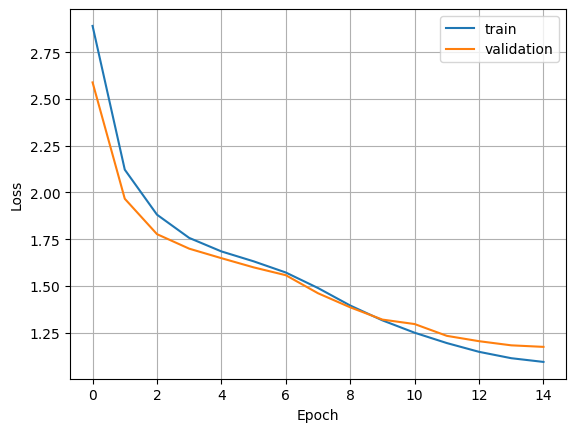
\includegraphics[width=0.8\textwidth]{./plots/recurrent_loss_per_epoch}
    \caption{Training and validation loss for the RNN model.}
    \label{fig:recurrent_loss_per_epoch}
\end{figure}

\begin{figure}[H]
\centering
\begin{subfigure}{.5\textwidth}
  \centering
  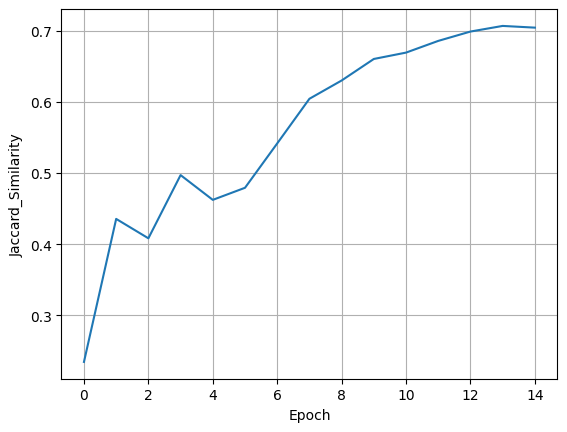
\includegraphics[width=.9\linewidth]{plots/recurrent_jaccard_similarity_per_epoch}
  \caption{Training Jaccard similarity per epoch}
\end{subfigure}%
\begin{subfigure}{.5\textwidth}
  \centering
  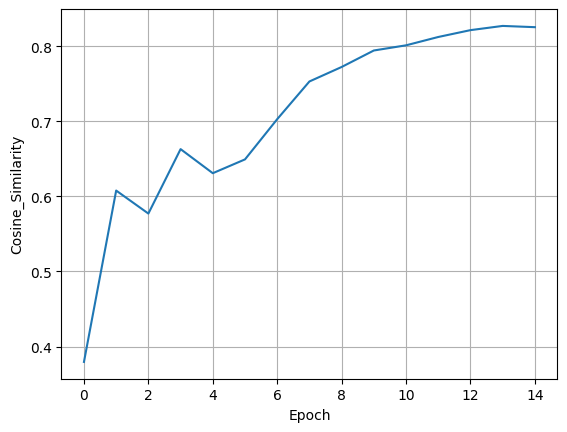
\includegraphics[width=.9\linewidth]{plots/recurrent_cosine_similarity_per_epoch}
  \caption{Training cosine similarity per epoch}
\end{subfigure}
\begin{subfigure}{.5\textwidth}
  \centering
  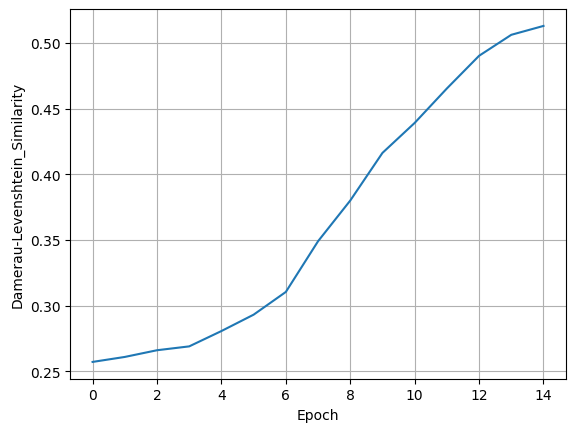
\includegraphics[width=.9\linewidth]{plots/recurrent_damerau-levenstein_similarity_per_epoch}
  \caption{Training Damerau-Levenstein similarity per epoch}
\end{subfigure}
\caption{Training similarity metrics per epoch for the RNN model.}
\label{fig:recurrent_similarity_per_epoch}
\end{figure}
The final testing metrics for the RNN were as follows:
\begin{itemize}
    \item Jaccard similarity: $0.7149$
    \item Cosine similarity: $0.8324$
    \item Damerau-Levenstein similarity: $0.5087$
    \item Loss: $1.1828$
\end{itemize}

\subsection{2.}
\begin{figure}[H]
    \centering
    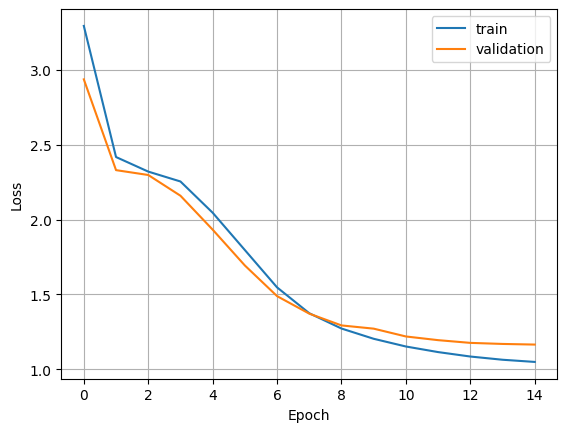
\includegraphics[width=0.8\textwidth]{./plots/transformer_loss_per_epoch}
    \caption{Training and validation loss for the RNN model.}
    \label{fig:transformer_loss_per_epoch}
\end{figure}

\begin{figure}[H]
\centering
\begin{subfigure}{.5\textwidth}
  \centering
  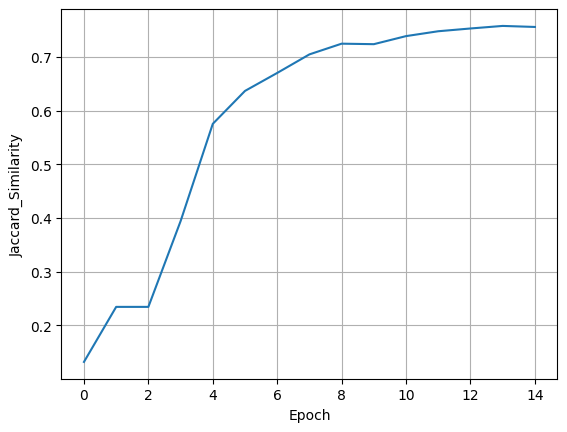
\includegraphics[width=.9\linewidth]{plots/transformer_jaccard_similarity_per_epoch}
  \caption{Training Jaccard similarity per epoch}
\end{subfigure}%
\begin{subfigure}{.5\textwidth}
  \centering
  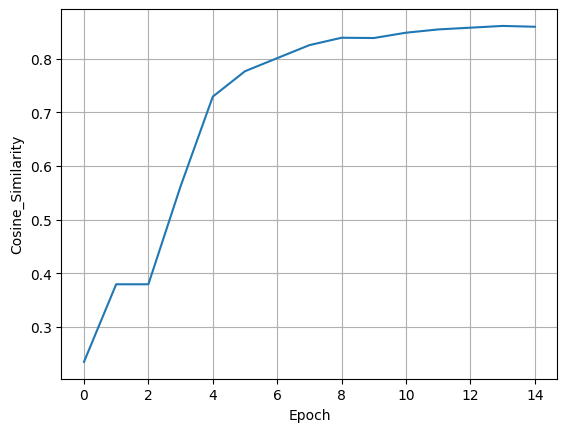
\includegraphics[width=.9\linewidth]{plots/transformer_cosine_similarity_per_epoch}
  \caption{Training cosine similarity per epoch}
\end{subfigure}
\begin{subfigure}{.5\textwidth}
  \centering
  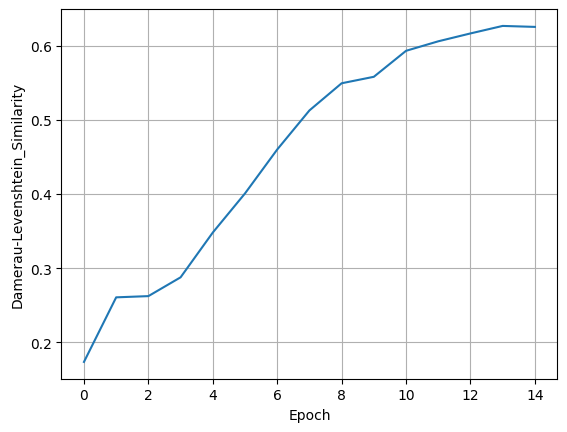
\includegraphics[width=.9\linewidth]{plots/transformer_damerau-levenstein_similarity_per_epoch}
  \caption{Training Damerau-Levenstein similarity per epoch}
\end{subfigure}
\caption{Training similarity metrics per epoch for the transformer model.}
\label{fig:transformer_similarity_per_epoch}
\end{figure}

The final testing metrics for the transformer were as follows:
\begin{itemize}
    \item Jaccard similarity: $0.7648$
    \item Cosine similarity: $0.8655$
    \item Damerau-Levenstein similarity: $0.6344$
    \item Loss: $1.1596$
\end{itemize}

\subsection{3.}
The LSTM decoder in question 1 uses a RNN to process the text input sequentially.
It maintains a hidden state and a cell state that encode the previous output and the context vector from the encoder.
The LSTM decoder generates the next output token based on the current input token, the hidden state, and the cell state.
It doesn't have direct access to the whole encoder output nor to the decoder outputs.

The attention decoder in question 2 uses a transformer to process the text input in parallel, without relying on recurrence.
It uses an attention mechanism to learn the relevance between the encoder output and the decoder input, and to produce a weighted context vector for each decoder input token.
The attention decoder generates the next output token based on the current input token, the context vector, and the previous decoder outputs.
It has direct access to the entire encoder output and the previous decoder outputs.
The non-reliance on recurrence allows the transformer to be run in parallel, which would explain the speed of training of 15 epochs of the transformer being about 10 minutes faster than the RNN.

The attention decoder in question 2 generally achieves better performance than the LSTM decoder in question 1.
This is because the attention decoder can capture the long-range dependencies and the global structure of the text input more effectively than the LSTM decoder.
The LSTM decoder can suffer from the vanishing gradient problem.
\subsection{4.}
\b{Jaccard similarity} is a measure of similarity between two sets.
It is the size of the intersection of the two sets divided by the size of the union of them.

\b{Cosine similarity} is a measure of similarity between two vectors.
It basically represents the angle between the two vectors.
The higher the cosine similarity, the smaller the angle and the more similar the two vectors are.

\b{Damerau-Levenstein similarity} is a measure of similarity between two strings.
It looks at the number of operations (inserion, deletion, transposition, substitution) needed to transform one string into the other.
It is calculated by subtracting the edit distance from the maximum possible distance, and dividing by the maximum possible distance.

All the similarity measures listed above can be applied to the text input and the text output of the model.
They differ in the way they measure the similarity.
The Jaccard similarity only compares the presence and non-presence of tokens.
It does not take into account the order and the frequency of the tokens.
The cosine similarity takes only into account the direction of the vectors but not their magnitude.
Whereas the Damerau-Levenstein similarity focuses on the amount of operations needed to transform one string into another.
Each of the similarity measures then differs in the way they are calculated and their respective values.
They can all be used depending on the application and the desired similarity measure.

\end{document}